\newcommand*{\memfontfamily}{pnc}%New Century Schoolbook 
\newcommand*{\memfontpack}{newcent}%(which comes in the T1 encoding),
\documentclass[pdftex,a4paper, 12pt, article, column, 
openany,extrafontsizes]{memoir}

\usepackage[italian]{babel}%localizzazione 

%\usepackage{lmodern}%latino moderno...
%\usepackage[T1]{fontenc}%.. codificato T1
%\usepackage{kpfonts} %altri font

\usepackage[utf8]{inputenc}
%ignore BOM (byte order mark) header for utf-8 file
%creato da quel fesso di kile! nei primi 3 byte
\DeclareUnicodeCharacter{FEFF}{} 
%\DeclareUnicodeCharacter{00A0}{~}

\usepackage[final]{microtype} % Less badboxes



\usepackage{amsmath,amssymb,mathtools} % Math


% layout 
\setlrmarginsandblock{0.1\paperwidth}{*}{1} % Left and right margin
\setulmarginsandblock{0.2\paperwidth}{*}{1}  % Upper and lower margin
\checkandfixthelayout

% \settrimmedsize{11in}{210mm}{*}
% \setlength{\trimtop}{0pt}
% \setlength{\trimedge}{\stockwidth}
% \addtolength{\trimedge}{-\paperwidth}
% \settypeblocksize{7.75in}{33pc}{*}
% \setulmargins{4cm}{*}{*}
% \setlrmargins{1.25in}{*}{*}
% \setmarginnotes{17pt}{51pt}{\onelineskip}
% \setheadfoot{\onelineskip}{2\onelineskip}
% \setheaderspaces{*}{2\onelineskip}{*}
% \checkandfixthelayout


%%% SECTIONAL DIVISIONS
%%%-----------------------------------------------------------------------------


\maxsecnumdepth{subsection} % Subsections (and higher) are numbered
\setsecnumdepth{subsection}

\makeatletter %
\makechapterstyle{standard}{
  \setlength{\beforechapskip}{0\baselineskip}
  \setlength{\midchapskip}{1\baselineskip}
  \setlength{\afterchapskip}{8\baselineskip}
  \renewcommand{\chapterheadstart}{\vspace*{\beforechapskip}}
  \renewcommand{\chapnamefont}{\centering\normalfont\Large}
  \renewcommand{\printchaptername}{\chapnamefont \@chapapp}
  \renewcommand{\chapternamenum}{\space}
  \renewcommand{\chapnumfont}{\normalfont\Large}
  \renewcommand{\printchapternum}{\chapnumfont \thechapter}
  \renewcommand{\afterchapternum}{\par\nobreak\vskip \midchapskip}
  \renewcommand{\printchapternonum}{\vspace*{\midchapskip}\vspace*{5mm}}
  \renewcommand{\chaptitlefont}{\centering\bfseries\LARGE}
  \renewcommand{\printchaptertitle}[1]{\chaptitlefont ##1}
  \renewcommand{\afterchaptertitle}{\par\nobreak\vskip \afterchapskip}
}
\makeatother

\chapterstyle{standard}

\setsecheadstyle{\normalfont\large\bfseries}
\setsubsecheadstyle{\normalfont\normalsize\bfseries}
\setparaheadstyle{\normalfont\normalsize\bfseries}
\setparaindent{0pt}\setafterparaskip{0pt}

%%% FLOATS AND CAPTIONS
%%%-----------------------------------------------------------------------------


\makeatletter                  % You do not need to write [htpb] all the time
\renewcommand\fps@figure{htbp} %
\renewcommand\fps@table{htbp}  %
\makeatother                   %

\captiondelim{\space } % A space between caption name and text
\captionnamefont{\small\bfseries} % Font of the caption name
\captiontitlefont{\small\normalfont} % Font of the caption text

\changecaptionwidth          % Change the width of the caption
\captionwidth{1\textwidth} %



%%% NEW COMMANDS
%%%-----------------------------------------------------------------------------


\newcommand{\p}{\partial} %Partial
% Or what ever you want

%%% TABLE OF CONTENTS
%%%-----------------------------------------------------------------------------


\maxtocdepth{subsection} % Only parts, chapters and sections in the table of 
%%contents
\settocdepth{subsection}

\AtEndDocument{\addtocontents{toc}{\par}} % Add a \par to the end of the TOC

%%% INTERNAL HYPERLINKS
%%%-----------------------------------------------------------------------------

\usepackage{hyperref}   % Internal hyperlinks
\hypersetup{
pdfborder={0 0 0},      % No borders around internal hyperlinks
pdfauthor={I am the Author} % author
}
\usepackage{memhfixc}   %

%%% THE DOCUMENT
%%% Where all the important stuff is included!
%%%-----------------------------------------------------------------------------

\author{N. Santi}

\title{Introduzione gentile alla relatività speciale}





\begin{document}



\frontmatter

\maketitle

\begin{abstract}
Albert Einstein formulò la sua teoria della relatività cent'anni fa ma ancora 
adesso non viene nemmeno insegnata nelle scuole elementari o medie. Nessuno ci 
capisce molto, in verità: sì, sappiamo che il tempo sia relativo ma non cosa 
significhi? Forse che ogni persona viaggia col suo tempo proprio, che non è 
possibile confrontare le esperienze degli uni con gli altri? Che il tempo 
passato con una bella ragazza/ragazzo sia più breve di quello passato seduto su 
una stufa accesa?

Non ci si capisce molto e il poco appreso in modo fortuito o frammentario non 
basta a ricostruire nemmeno le basi della bella e strana teoria della 
relatività.

Il punto è che per comprenderla veramente serve la matematica: non quella usata 
solitamente nei libri di testo per nascondere il vero significato delle cose 
dietro una selva di calcoli brigosi. No, quello che serve è quel minimo di 
matematica che ci aiuti a capire cosa sia lo spazio-tempo, a toccarlo con dei 
calcoli facili solo per farsi aiutare nella comprensione.

Lo scopo di questo articolo è quindi quello di illustrare la relatività speciale 
con lunghi discorsi e un solo esempio matematico basato sulle sole quattro 
operazioni, quelle apprese nelle scuole elementari. Per i più temerari esiste 
anche un'appendice che richiede una minima conoscenza di algebra, del tipo 
appreso all'ultimo anno delle scuole medie.

La speranza è quella di riuscire a divulgare a quante più persone possibile i 
fondamenti dell'universo in cui ci è capitato di vivere e fornire 
un'introduzione gentile per gli studenti che intendano iniziare lo studio della 
fisica relativistica.

\end{abstract}

\clearpage

\tableofcontents*
\clearpage
\frontmatter


\chapter{Relatività Galileiana}

\section{Stato naturale di un corpo}

Secondo Aristotele, filosofo dell’antica Grecia,  lo stato naturale di un corpo è quello di quiete: se niente lo spingesse prima o poi si fermerebbe e così resterebbe in eterno. Siete d’accordo con lui? Sì? No? Provate a guardate, per esempio, il pallone fermo nel campo, la slitta carica di blocchi di marmo e l’acqua nel bicchiere. Tutto qui sulla terra sembra confermare le parole di Aristotele.

Purtroppo però quelle parole sono sbagliate: se la pensate come lui dovreste fare un upgrade di poco meno di 2 mila anni per  conoscere il genio toscano di Galileo Galilei il quale ci insegna che un corpo lasciato a sé stesso, cioè senza nessuna forza che agisca su esso, mantiene costante la propria velocità per sempre. Quindi, se nessuno lo spingesse più ed era fermo, fermo rimarrebbe proprio come sostiene Aristotele. Se però era in movimento continuerebbe a muoversi alla stessa velocità, senza accelerazioni o decelerazioni lungo una linea retta, per sempre. 

Questo tipo di moto, chiamato rettilineo uniforme, sembra quindi essere il vero stato naturale di un corpo. Sulla terra tutto sembra contraddire Galileo perché c’è sempre qualche agente frenante, cioè qualche forza che infine ferma la palla, la slitta o l'acqua nel bicchiere: ad esempio l’attrito dell’aria, della terra e la gravità stessa. Per avere un'immagine mentale a cui aggrapparvi pensate al meteorite nello spazio, lontano da qualsiasi pianeta: immaginatelo nel suo viaggio solitario, rettilineo e senza accelerazioni in eterno senza bisogno di nessuna forza che agisca su esso.

Newton ha saccheggiato questo principio importantissimo da Galileo e l'ha chiamato, assiomaticamente, \textit{primo principio della dinamica}, o semplicemente \textbf{principio d’inerzia}: ci ricorda come i corpi siano inerti, continuano a mantenere la velocità che avevano quando si smette di applicare loro una forza.


\section{Relatività galileiana, 1}

I due stati quindi, quello di quiete e quello di moto rettilineo uniforme, sono del tutto indistinguibili da un punto di vista fisico, e questo è il punto importante che apprenderemo adesso: se lanciate in alto una palla su un treno fermo vi ricadrà in mano, se fate lo stesso su un treno immaginario in moto rettilineo uniforme che viaggi a $200 km/h$ succederà la stessa identica cosa. Versate l’acqua nel bicchiere questa non scorre indietro per il fatto che il treno si muova ma continua a cadere perfettamente in verticale nel bicchiere come quando siete fermi.

Nulla tradisce lo stato di moto senza accelerazioni, nessun esperimento consente di distinguerlo dallo stato di quiete  e questo è una realtà di cui convincersi profondamente prima di affrontare la relatività di Einstein. Approfondiamo un poco l'argomento.

La palla è ferma in mano al viaggiatore, per lui non si muove, mentre la stessa palla, per una osservatrice ferma alla stazione si muove come il treno a $200 km/h$. La palla lanciata sul treno, dal fondo di un vagone verso la locomotiva viaggia a $30 km/h$ per i passeggeri del treno e a $230 km/h$ per la donna ferma alla stazione. Il calcolo è facile, basta sommare alla velocità della palla (per i passeggeri) quella del treno, $30+200=230$. 

Una palla lanciata invece nella direzione opposta viaggerà sempre a $30 km/h$ per i passeggeri ma a $170 km/h$ per la donna in stazione. In questo caso si sottraggono le velocità $200-30=170$.

La velocità è dunque un concetto relativo, come a dire che lo stato di quiete o di moto dipendono dall’osservatore e nessuno dei due sbaglia. 

Questo è il secondo punto da assimilare prima di procedere (il primo era l'indistinguibilità dei due stati di moto per chi li sperimenta). Se pensate che sia un ragionamento cervellotico questo della relatività, se non lo ritenete una realtà fisica vi sbagliate di grosso. Riflettete su questo: la palla lanciata delicatamente ($1 km/h$) tra due passeggeri del solito treno può anche essere presa al volo anche da un bambino piccolo, non gli procurerà alcun male. Un grosso male invece  sentirebbe quel bambino se  per lui la palla viaggiasse a $201 km/h$ orari, come ritiene la donna in stazione.

Rifletteteci sopra fino a domani, quando vi convincerete dello stato delle cose potrete procedere.

\section{Relatività galileiana, 2}

Se lo stato di quiete o di moto rettilineo uniforme sono indistinguibili da chi lo sperimenta allora abbiamo bisogno di un osservatore esterno per discriminare. La scelta dell’osservatore può portare a risultati diversi, come sappiamo: per qualcuno ci muoviamo, per altri stiamo fermi.

Senza osservatori esterni non esisterebbe neppure il concetto di moto. Non ci credete vero? Immaginate allora di essere soli nello spazio profondo, senza alcuna cosa attorno a voi: il moto esisterebbe? No, non esisterebbe senza un punto fisso, altro rispetto a noi. Se poi state pensando che anche in questo spazio potreste muovere le braccia vi invito a riflettere che muovere le braccia rispetto al corpo significa già avere un punto di riferimento: il corpo.

Per annullare completamente il concetto di moto dovete pensare ad un piccolissimo oggetto indivisibile senza nulla attorno: il concetto di movimento non esisterebbe proprio per questa minuscola pallina.

Prima di procedere dovete concordare sulla mia prossima affermazione: è la terra e muoversi attorno al sole. 

Il cardinale Bellarmino, che costrinse Galileo alla famosa abiura, non aveva torto da un punto di vista scientifico. Aveva invece torto da vendere imponendo con la violenza la visione di un Chiesa timorosa di perdere la propria egemonia. Si sbagliava anche sostenendo che Galileo avesse torto, la terra gira attorno al sole almeno quanto il sole giri attorno alla terra. Il moto è un concetto relativo.

Siete d’accordo? Se sì, procedete.


\section{Esperimento della pallina, 1}

In pochi paragrafi siamo quindi giunti attorno al 1600 apprendendo qualcosa del monumentale lavoro di Galileo: sappiamo che il moto, e quindi la velocità, sono concetti relativi. Anche la traiettoria lo è: la palla lanciata in verticale sul treno descrive una traiettoria dal basso verso l’alto e poi al contrario: una semiretta verticale per i passeggeri. Per la donna alla stazione però disegna una parabola, non ricade dove era stata lanciata perché il treno nel frattempo si è spostato in avanti a $200 km/h$.

Adesso dobbiamo formalizzare quando appreso in modo da passare da una descrizione della realtà, quella dei passeggeri, ad un'altra, quella della donna sulla pensilina. Lo faremo con un grafico molto semplice che useremo poi anche per descrivere la relatività di Einstein. Le due descrizioni della realtà si chiamano, tecnicamente, sistemi di riferimento\footnote{Ciascuno sistema di riferimento si muove rispetto all’altro in moto rettilineo uniforme a $200 km/h$ (la velocità del treno), si dicono perciò sistemi di riferimento inerziali e sono gli unici che studieremo.}  e servono per descrivere lo stesso evento in modi diversi: ogni evento avviene in una dato momento e in un punto preciso dello spazio per cui il sistema di riferimento della donna indicherà tempi e spazi con i simboli $(t,x)$ mentre quello dei passeggeri con i simboli $(t',x')$.

Vogliamo descrive nei due sistemi di riferimento lo stesso esperimento, visto da due punti di vista diversi: l'esperimento sarà tra i più stupidi mai escogitati, temo, e consisterà nel descrivere il moto di una pallina lanciata dall'ultimo vagone del treno contro la locomotiva. Ce la facciamo facile immaginando un treno formato da un solo vagone/locomotiva, senza ostacoli sulla strada della nostra pallina.

Diciamo poi il treno sia lungo  $c$, una distanza qualsiasi, ad esempio $20$ metri. Anzi, semplifichiamo ulteriormente diciamo che il treno è lungo $1$, un'unità di misura costruita apposta per noi, per cui $c=1$.  Inoltre diciamo che il treno si muova ad una velocità pari a $v$ che poniamo uguale a metà della sua lunghezza del treno $c/2$ (si legge $c$ mezzi).  Vuole dire che ogni secondo il nostro treno copre una distanza pari a metà della sua lunghezza, se fosse lungo $20$ metri ogni secondo ne percorrerebbe $10$ viaggiando quindi a $10$ metri al secondo, si indica così $v=10m/s$. Si dice che un'immagine valga cento parole per cui:

\begin{figure}[h!]
 \centering
 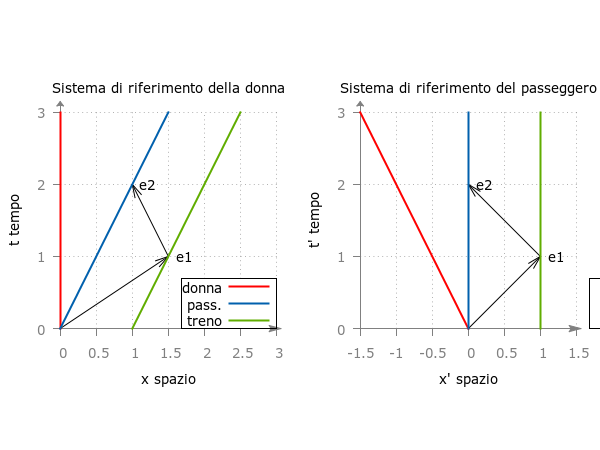
\includegraphics[scale=0.7]{figure/fig4}
 \caption{Esperimento della pallina}
\end{figure}

Non spaventatesi e continuate a leggere, iniziamo dal grafico di sinistra: rappresenta l'esperimento nel sistema di riferimento della signora. Dal suo punto di vista lei stessa è immobile, rimane sempre nella posizione $x=0$ per ogni tempo ed è quindi rappresentata dalla linea verticale rossa, quella più a sinistra. Nell'istante $0$ incrocia il passeggero seduto in coda al treno per cui, in quel momento, i due saranno entrambi nella posizione $0$ e poi il passeggero si allontana lungo la linea blu. La locomotiva del treno è sempre $c=1$ più avanti rispetto al passeggero perché il treno stesso è lungo $c$: la posizione della testa del treno è rappresentata dalla linea verde, quella più a destra.

Lo stesso esperimento è diverso invece per il passeggero, il cui sistema di riferimento è rappresentato nel grafico a destra. Dal suo punto di vista lui è quello fermo, indicato la linea centrale, sempre in blu. Anche la locomotiva per lui è ferma alla distanza $c$ da lui da cui la linea verde a destra. In questo sistema di riferimento si muove solo la signora e la pensilina su cui si trova: per il passeggero infatti la donna si allontana da lui a velocità $v$\footnote{Tecnicamente la velocità sarebbe $-v$, dove il segno meno indica che la donna si muove nella direzione opposta al treno.} come vediamo nella linea rossa a sinistra.

Riepilogando: la linea rossa, che si chiama linea di universo, rappresenta la donna, mentre il treno si estende dalla linea blu, la coda, a quella verde, la locomotiva.

Soffermatevi il tempo necessario per comprendere questi grafici in cui troviamo rappresentati i concetti fino a qui espressi a parole.

\section{Esperimento della pallina, 2}

Pronti a riprendere il nostro esperimento? Bene, diciamo che quando la coda del treno passa davanti alla donna alla stazione, il passeggero seduto proprio in fondo al treno lancia la palla nella direzione di marcia: ci chiediamo quando la palla tocchi la testa del treno? Quando rimbalzando indietro torna in mano al passeggero? E soprattutto: per i due sistemi di riferimento, quello della donna e quello del passeggero, come saranno diversi questi calcoli?

Ci manca un dato? Sì, sappiamo che il treno è lungo $c=1$ e che viaggia a $v=c/2$ ma a quando viaggia la pallina per il passeggero sul treno? Diciamo, sempre per facilitarci il lavoro, $c=1$: cioè ogni secondo la pallina percorre la lunghezza del treno (sì,viaggia parecchio veloce questa pallina).

Abbiamo promesso di usare solo le quattro operazioni e così faremo: con dati così semplici il calcolo è davvero facile. Per il passeggero seduto in fondo al treno la palla, che ogni secondo percorre $c$, ci mette quindi un solo secondo a raggiungere la locomotiva distante $c$.  Un secondo per andare e un altro secondo per tornare indietro.

Possiamo vederlo bene nella figura 1, grafico di destra: la freccia che esce dall'origine rappresenta il percorso della pallina che dopo $1$ secondo raggiunge la testa del treno rappresentata dalla linea verde. Possiamo chiamare questo evento $e1$ intendendo sia  quando ($1$ secondo) sia dove (posizione $c$) la pallina incontra la locomotiva. Il viaggio di ritorno della pallina è rappresentato dalla seconda freccia che da $e1$ torna verso il passeggero, linea blu, intercettandolo dopo $1$ secondo. Quel momento e quel luogo lo chiamiamo evento $e2$.

Lo stesso esperimento è descritto in modo molto diverso dalla signora sulla pensilina: per lei la testa del treno si sposta ad una velocità pari a $v=c/2$, linea verde del grafico a sinistra, per cui la pallina dovrà rincorrerla. Per la signora la pallina si muove ad una velocità pari a $c+v$, per quanto abbiamo detto nei paragrafi precedenti. 

Quanto ci mette a raggiungere la testa del treno?  Che domanda scontata direte voi, non serve nemmeno fare i calcoli: se quando la pallina tocca la testa del treno l’orologio del passeggero segna $1$ secondo, anche quello della donna, per lo stesso evento $e1$, dovrà segnare lo stesso tempo. Per cui la pallina tocca la locomotiva dopo $1$ secondo. 

Avete ragione... ma solo per ora come vedremo più avanti. In ogni caso per velocità così ridotte anche per la donna la pallina ci mette un secondo a raggiungere la testa del treno e uno a tornare indietro. Il percorso della pallina è rappresentato anche qui dalle due frecce nel grafico a sinistra. 

Se però i due sistemi di riferimento concordano sui tempi non concordano però sulle velocità o sullo spazio percorso: riassumiamo nella prossima tabella i nostri risultati.

\begin{center}
\begin{tabular}{>{\itshape}l >{\itshape}c >{\itshape}c }
\toprule
            & \textbf{donna} & \textbf{passeggero} \\
velocità treno            & $v$   & $0$  \\ 
velocità pensilina        & $0$   & $-v$  \\
velocità pallina          & $c+v$ & $c$  \\
secondi dell'esperimento  & $2$   & $2$  \\
distanza percorsa dalla pallina   & $2v$  & $2c$  \\
lunghezza del treno       & $c$   & $c$  \\
\bottomrule
\end{tabular} 
\end{center}


Nei due sistemi di riferimento la velocità relativa di treni e pensilina coincide, $v$. Anche i tempi coincidono, ma non la velocità della pallina: misurandola con qualsiasi mezzo per la donna sarebbe maggiore che per il passeggero. Quindi se la velocità è maggiore, ma i tempi sono li stessi tempi, se ne deduce che la pallina ha percorso un tragitto più lungo per il donna rispetto a quanto creda il passeggero.

Facciamo un ultimo sforzo per verificare la lunghezza del treno per la donna sulla pensilina: sappiamo che dopo $1$ secondo la locomotiva  si trova alla distanza $v+c$. La parte coda del treno invece si trova, dopo $1$ secondo, alla distanza $v$. Quindi otteniamo che il treno sia lungo $c$ e tutto quadra.

Rifletteteci un po’ sopra prima di procedere. Se vi va e vi ricordate la semplice algebra della terza media  saltate  all’appendice per provare a rifare i calcoli assieme.


\section{Relatività galileiana, 3}

Questo è un paragrafo di tutto relax: faremo solo dei disegnini per rappresentare l’esperimento visto in precedenza e passare da un sistema di riferimento ad un altro, senza fare calcoli ma limitandosi a guardare.

Ritroviamo in entrambi i grafici gli eventi $e1$, la pallina raggiunge la locomotiva e $e2$, quando questa torna in mano al passeggero. Le frecce qui non rappresentano più il percorso della pallina ma ci mostrano come, dato un evento, se ne possano trovare le coordinate cioè quando accade e dove accade. A sinistra abbiamo la condizione usuale, quella imparata a scuola, per cui dall'evento scendiamo in verticale per trovare la posizione, $x=1.5$, oppure in orizzontale per ottenere il tempo $t=1$. In pratica muoviamo dall'evento agli assi cartesiani (in blu nel grafico).

\begin{figure}[h!]
 \centering
 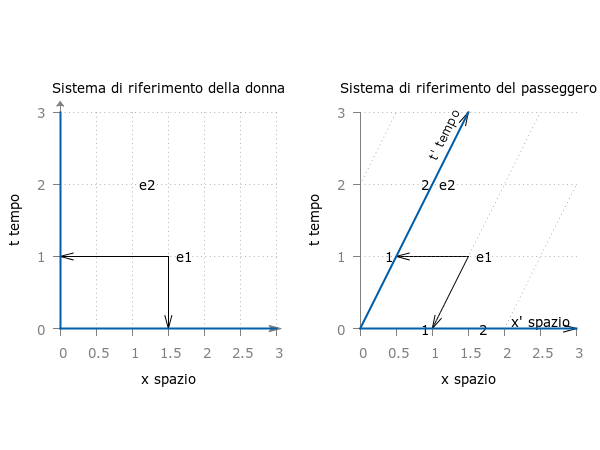
\includegraphics[scale=0.7]{figure/fig5}
 \caption{relatività galileiana}
\end{figure}

Per ottenere le coordinate $x'$ e $t'$ dello stesso evento $e1$ dal punto di vista del passeggero si possono tenere fermi i punti degli eventi però utilizzando degli assi diversi, visibili sempre in blu nel grafico di destra. Anche in questo caso ci muoviamo dall'evento $e1$ verso gli assi e leggiamo lì sopra le coordinate $x'=1$ e $t'=1$.

Useremo queste rappresentazioni per avere sott'occhio contemporaneamente i due sistemi di riferimento in un solo grafico e semplificarci i ragionamenti. \footnote{Il sistema di assi di destra chiaramente non è cartesiano perché gli assi non sono tra loro ortogonali. C'è però di peggio: la distanza dall'origine per l'asse $t'$ non riporta il tempo ma una sua funzione lineare, $t'\sqrt{1+v^2}$. Non ci cureremo troppo di questi dettagli limitandoci a leggere le etichette sui nuovi assi obliqui senza chiederci come si misurino.}

Provate da soli a riportare nel grafico a sinistra gli assi $x'$ e $t'$ in modo da avere in un solo colpo d'occhio entrambi i sistemi di riferimento.

\section{Sincronizzare gli orologi}

Ovvero come misurare gli intervalli di tempo. Con un cronometro rispondete? Be’, certo. Però dovremo domandarci come faccia il passeggero, seduto a metà treno, a sapere che esattamente dopo un $1$ la pallina tocca la testa del treno? Lui si trova da un’altra parte in quel momento quindi come può esserne certo?

Pensate ad un modo sicuro per riuscirci, anche se stravagante, non importa.

Pensato?

Si potrebbe fare così: nel momento in cui incrocia la donna sulla banchina il passeggero potrebbe sincronizzare due orologi con quello di lei e poi, successivamente, potrebbe andare a mettere uno dei due nella testa del treno. A quel punto ritorna al suo posto, lancia la palla e quando questa colpisce la testa del treno scatta una foto o guarda direttamente con un binocolo l’orologio in modo da sapere con esattezza l’orario in quel momento. La stessa cosa può fare anche la donna sincronizzando orologi quando incroci il passeggero e poi piazzarli lungo il binario per poi guardare quello vicino al luogo in cui la palla raggiungerà la testa del treno. Oppure anche qui fare delle foto dei vari eventi. 

Esiste però un modo più generale per sincronizzare gli orologi che evita di spostarli \footnote{Come scopriremo spostare i orologi sincronizzati significa... che non sono più sincronizzati!}: prima si dispongono dove si crede, a metà treno, sulla locomotiva, sulla pensilina, ovunque insomma. Poi quando il passeggero incroci la donna ferma alla stazione si azzerano gli orologi che hanno in mano e contemporaneamente si lancia un raggio di luce verso gli altri orologi. Dal momento che la velocità della luce è \textit{tragicamente} costante, conoscendo la distanza degli orologi, si sa esattamente dopo quanti secondi saranno raggiunti dal raggio e in quel momento inizieranno a muoversi. Non è difficile: diciamo che la luce percorra una distanza pari a $c$ ogni secondo. L'orologio che si trovi alla distanza $c$ dal passeggero sarà raggiunto dopo $1$ secondo e in quel momento segnerà $1$ e inizierà a contare il tempo. L'orologio che si trovi alla distanza $2c$ dal passeggero sarà raggiunto dopo $2$ secondo e in quel momento segnerà $2$ e inizierà a contare il tempo.  

Semplice no? Questo modo di sincronizzare gli orologi tra l'altro è l'unico possibile sulle grandi distanze, tipo quelle interplanetarie. 

Ricapitolando, una volta sincronizzati gli orologi segneranno tutti la stessa ora. Ora questo paragrafo vi sembrerà ovvio, ma sono pronto a scommettere che ci tornerete sopra quando nella prossima sezione discuteremo la relatività del tempo.


\section{Misurare le lunghezze}

Per misurare la lunghezza di un oggetto come si procede? Si pone un capo del metro su un lato, l'altro capo dalla parte opposta e si legge la lunghezza. Da notare come questa questa operazione deve essere simultanea: se quando leggo la misura su un capo l'altro non coincide più con l'estremità dell'oggetto da misurare non sto facendo un buon lavoro. 

\begin{figure}[h!]
 \centering
 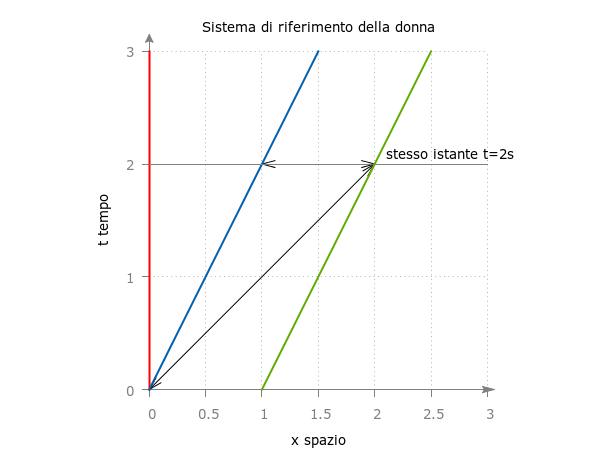
\includegraphics[scale=0.7]{figure/fig7}
 \caption{relatività galileiana}
\end{figure}


Quest'ultima informazione è importante anche se non ora non ci sembra: il fatto che le distanze tra i due estremi dell'oggetto debbano essere misurate \textit{simultaneamente}, nello stesso istante, ci procurerà qualche problema nei prossimi paragrafi. Nella figura 3 si vede chiaramente che misurando in istanti diversi (la linea obliqua nera) si ottiene una lunghezza diversa rispetto a misurare nello stesso istante (linea orizzontale nera): la lunghezza del treno risulterebbe maggiore di $1$ considerando gli estremi in momenti diversi. 

Infine, sapete immaginare un metodo più generale per misurare le distanze? Per oggetti lunghissimo o lontani da noi? No? Non avete letto bene il paragrafo precedente bene allora. Tornate indietro?

Usando la luce? Esatto: si lanciano due raggi in modo che raggiungano \textbf{contemporaneamente} gli estremi dell'oggetto e poi si aspetta che ritornino indietro. Vediamo un grafico per capire meglio la situazione:

FIG MISURARE LUNGHEZZE

Oh bene, a questo punto disponiamo di tutti gli elementi per comprendere facilmente la teoria della relatività speciale di  Einstein. Partiamo!

\chapter{Relatività Speciale}

\section{Un problema luminoso}

La luce non si comporta secondo la relatività galileiana: ecco, questa è la cruda verità. Macchine, proiettili, missili, ogni cosa sembra rispettare le indicazioni di Galileo tranne la luce\footnote{In realtà scopriremo come tutte le cose \textbf{non} rispettino la relatività galileiana ma ci vadano solo vicino quando le velocità siano piccole rispetto alla luce. In altri termini la relatività galileiana approssima il vero comportamento dei corpi in movimento: minore la velocità e minore sarà l'approssimazione.}.

Per evitare fraintendimenti iniziamo dai dati di fatto tornando sul nostro treno: se  sparassimo un raggio di luce invece che lanciare la nostra cara pallina ci ritroveremo subito in un bel guaio perché la velocità della luce sarebbe la stessa anche per la signora sulla pensilina. 

Sì, è assurdo e sì, il treno si muove eppure le cose stanno così.

Ripeto, la velocità della luce misurata sul treno in movimento\footnote{In movimento rispetto alla donna ferma alla banchina.} coinciderebbe con quella misurata dalla signora sulla pensilina: da qui muove l’opera di Einstein cercando di spiegare questa anomalia. 

\begin{figure}[h!]
 \centering
 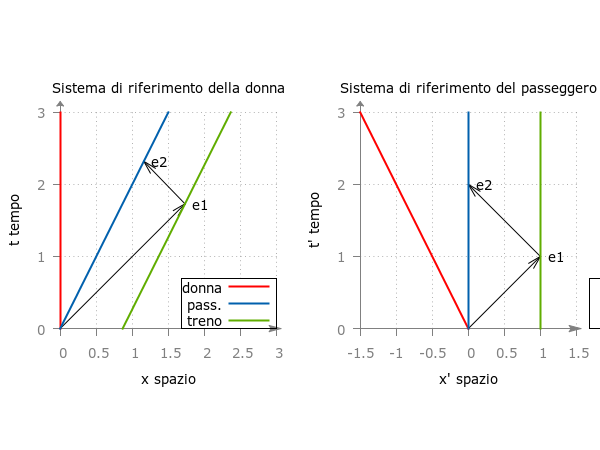
\includegraphics[scale=0.7]{figure/fig8}
 \caption{relatività galileiana}
\end{figure}



Studieremo la cosa da diversi punti di vista, prima però rifacciamo l’esperimento utilizzando la luce invece che una pallina per avere dei dati sotto mano: useremo sempre gli stessi simboli per non confonderci, modificandone però il significato. Ad esempio il treno sarà sempre lungo $c$ però questa volta $c$ indica la distanza percorsa dalla luce in un secondo, qualcosa come $299.792.458$ metri, quasi $300$ mila chilometri al secondo! Dobbiamo utilizzare grandezze così enormi altrimenti non riusciamo ad inquadrare facilmente il punto su cui ragioniamo. La velocità del treno sarà ancora $v=c/2$, $150.000$ metri ogni secondo: con una velocità del genere possiamo confidare di non avere più treni in ritardo, forse;-)

Facciamo i conti: per il passeggero tutto rimane invariato, il raggio di luce impiega $1$ secondo a percorrere la distanza $c$, quindi tutto come prima: in $2$ secondi torna indietro. Evviva!

Per la signora sulla pensilina però la luce emessa dal treno si muove a $c$, non più a $c+v$ come dovrebbe accadere secondo Galileo. Per  inseguire la testa del treno che si allontana a velocità $v$ il raggio di luce ci mette più di un secondo. Ripeto: se la testa del treno stesse ferma il raggio di luce ci metterebbe $1$ secondo a raggiungerla, ma si muove, si allontana quindi ci mette qualcosa di più di un secondo, precisamente: 1,73 secondi.\footnote{Nell'appendice, per chi ha voglia, si possono seguire i calcoli e scoprire che il tempo trascorso è $c^2/\beta$ dove $\beta= c-v$, data la velocità del treno è una costante che ritroveremo in diversi punti del nostro ragionamento: tanto vale fare la conoscenza e notare come $\beta<1$ dal momento che ogni oggetto si muove ad una velocità $v$ minore di quella della luce $c$.}. Anche a fare il giro completo ci impiega più di due secondi, 2,32 per l'esattezza. Nel grafico questo disallineamento degli eventi $e1$ e$e2$ è particolarmente evidente: nel modello galileiano differivano solo per lo spazio adesso invece anche i tempi non coincidono.

Possiamo già fermarci e riflettere sul fatto che lo stesso accadimento, lo stesso evento, avvenga dopo un secondo per il passeggero ma più tardi per la signora sulla pensilina: lo stesso \textbf{identico} evento non è più simultaneo per i due osservatori. 

Il trionfo dell'assurdità: benvenuti nell'universo relativistico in cui, d'altronde, vivete dal giorno in cui siete nati!

\section{Relatività del tempo, 1}

Magari abbiamo sbagliato i calcoli, può essere. Così hanno pensato i fisici di fronte ai risultati di molti esperimenti anche precedenti alla formulazione di Einstein: non è possibile che lo stesso evento avvenga in tempi diversi. L'esperienza di tutti i giorni ci dice esattamente il contrario... proprio come l'esperienza quotidiana dava ragione ad Aristotele circa lo stato naturale dei corpi.

Però Aristotele aveva torto, come sappiamo, e Galileo ragione, cosa che ci porta ad accettare la realtà anche se apparentemente strana e priva di senso. Quindi torniamo ai fatti: l'evento definibile come “il raggio di luce tocca la testa del treno” che chiamiamo $e1$ si comporta in modo strano, avviene prima per il passeggero e poi per la signora. Il problema non è $e1$, ma la velocità della luce che rimane costante per la donna, come abbiamo visto. Da questa inspiegabile invarianza ne deriva che il tempo trascorso per la donna, indichiamolo con $\Delta t$ è più lungo del tempo trascorso per il passeggero $\Delta t'$, per lui il tempo scorre più lento, a quanto pare. Se la signora potesse sbirciare nel treno in movimento vedrebbe ogni cosa al suo interno muoversi al rallentatore, compreso il battito cardiaco del passeggero.

Lo so, non ci credete: nessuno d'altronde credeva ad Einstein. In molti, per molti hanno hanno tentato di confutare in tutti i modi sperimentabili la sua teoria. Una volta hanno sincronizzato due orologi atomici, i più precisi di cui disponiamo, e piazzato uno dei due su un aeroplano che ha voluto in giro per il mondo. Il punto qui è che si muoveva rispetto al gemello fermo anche se a velocità piccole rispetto a quelle della luce. Eppure, tornato alla base, i due orologi non erano più sincronizzati: il viaggiatore era in ritardo rispetto a quello fermo\footnote{L'aereo girava intorno alla terra quindi non si muoveva in moto rettilineo uniforme: i discorsi sulla relatività che faremo più avanti quindi valgono solo per metà ;-)}.

Quindi il tempo è un concetto relativo come la velocità galileiana, come l'alto ed il basso, come il vicino o il lontano. Rifletteteci sopra un po' prima di procedere... intanto vi intrattengo con un altro esempio preso dalla realtà: parliamo di GPS, quel sistema che consente al vostro navigatore o cellulare di dirvi dove vi trovate sulla terra con un'ottima approssimazione. Forse non sapete che si basa su una rete di 24 satelliti che gravitano attorno al mondo in modo tale che almeno quattro siano sempre visibili da ogni luogo terrestre. Sono come dei fari per i marinai: ricevendo il loro segnale, sapendo quando lo hanno inviato e quanto tempo ci abbiamo messo a riceverlo riusciamo a scoprire quando siamo distanti da loro. 

Il punto è che l'accuratezza nel misurare il tempo è fondamentale per il funzionamento di tutto il sistema ed è qui che entra in gioco Einstein: in questi satelliti ci sono degli orologi che, udite udite, perdono tempo rispetto a quelli a terra secondo le predizioni della teoria che stiamo studiando\footnote {E anche per gli effetti di dilatazione del tempo dovuti alla gravità che non studieremo ma sono spiegati sempre da Einstein nella Teoria della Relatività Generale.}. Questo errore è compensato in modo da sincronizzare gli orologi e grazie ad Einstein abbiamo i navigatori satellitari! 

Meditate.

\section{Relatività di Einstein}

Parlando di relatività galileiana abbiamo imparato ad utilizzare un metodo grafico per ricavare le coordinate del passeggero $t',x'$ restando nella rappresentazione della signora. Possiamo fare lo stesso anche occupandoci della relatività di Einstein.


\begin{figure}[h!]
 \centering
 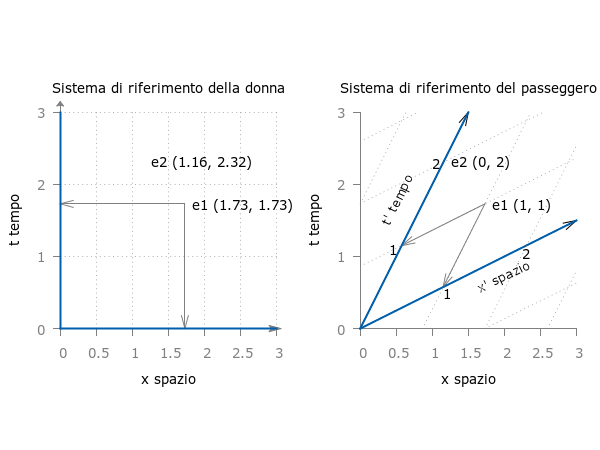
\includegraphics[scale=0.7]{figure/fig10}
 \caption{relatività galileiana}
\end{figure}

I due eventi si trovano in entrambi i grafici nella stessa posizione, il procedimento per ottenere le coordinate rimane il solito ovvero si seguono le frecce fino ai nuovi assi: l'unica incredibile differenza è che qui, dato un evento, passando da un sistema all'altro non si modifica solo la posizione nello spazio ma anche il tempo. Vi invito a notare l'asse $x'$ che è l'insieme di tutti gli eventi nell'universo per cui, per il passeggero, il tempo vale $t'=0$. In altre parole sono tutti gli eventi contemporanei al momento della sincronizzazione per il passeggero. Vi prego di notare come non sia più una curva piatta ma abbia un'inclinazione pari alla velocità $v$ del treno.

Sopra questo asse, e parallele a questo, abbiamo invece altre linee che raggruppano eventi contemporanei: avremo la linea di tutti gli eventi quando il tempo è pari a $1$ secondo, pari a $2$ e così via, una sopra l'altra (sono le linee tratteggiate parallele a $x'$.

Questa differenza di prospettiva per cui per la signora gli eventi contemporanei sono indicati da linee piatte e per il passeggero invece sono inclinate porta al risultato che, gli stessi eventi, hanno tempi diversi per i nostri due personaggi.

Provate ad allenarvi trovando le coordinate per $e1$ e $e2$ per i diversi sistemi di riferimento utilizzando un unico grafico.


\section{Spazio-tempo}

Nel nostro esperimento relativistico gli orologi sul treno sono sincronizzati con quello del viaggiatore utilizzando un raggio di luce, come abbiamo spiegato nella sezione precedente. Lo stesso è stato fatto per gli orologi sulla banchina: sono tutti coincidenti con quello della donna.

\begin{figure}[h!]
 \centering
 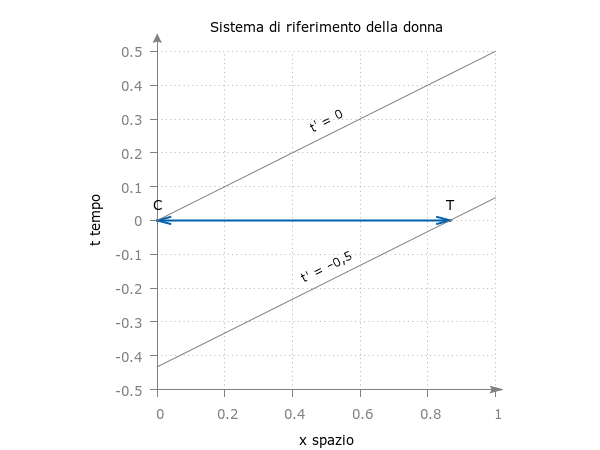
\includegraphics[scale=0.7]{figure/fig9}
 \caption{relatività galileiana}
\end{figure}

Nella figura qui sopra il treno, al momento della sincronizzazione degli orologi, è rappresentato con la linea blu orizzontale \footnote{I più attenti noteranno che il treno sia un po' più corto di $c$: non è uno sbaglio ma ne parleremo più avanti.} che va dall'evento $C$, coda del treno incrocia banchina, all'evento $T$, testa del treno incrocia fine banchina. Ricordo che il passeggero si trova in coda al treno.

Le due linea parallele sopra è sotto il treno nel nostro grafico le abbiamo conosciute nel paragrafo precedente e mostrano rispettivamente gli eventi che per il passeggero sono contemporanei a $t'=0$ e $t'=-0,5$. Tra queste due ci sono infinite linee parallele per i secondi tra $-0.5$ e $0$.

Il dato che emerge è che dopo la sincronizzazione avvenuta in $C$ per la donna, nello stesso istante, anche l'orologio in $T$ segna $0$. Normale, direte voi: già peccato però che potendo vedere dentro il treno in $T$ vedremo l'orologio del passeggero segnare un tempo precedente a zero,  $-0.5$!

La lezione è che con la caduta del tempo assoluto non esiste più uno spazio ed un tempo unico per tutti ma una cosa che è l'unione dei due, chiamata spazio-tempo costituita in ogni punto nelle spazio E nel tempo. Si tratta dei nostri eventi, come $C$ e $T$.

Il tempo e lo spazio sono mescolati in quantità diverse per osservatori diversi ma lo spazio-tempo è invariante per tutti.

Riflettete su questa importante lezione: il punto è che eventi simultanei per un osservatore non lo sono per un altro (le linee parallele piatte contro quelle inclinate). Ne deriva ad esempio che spostandosi lungo il treno nello stesso istante $t=0$ (per la signora) vedremo orologi sul treno avere orari diversi, via via minori, perché per il passeggero quegli eventi non sono contemporanei a $C$.


\section{Relatività del tempo, 2}

Il moto, lo abbiamo visto, è un concetto relativo sotto diversi punti di vista. Non solo dipende dagli osservatori, ma è anche del tutto impossibile capire per uno di loro se sia in moto (rettilineo uniforme) oppure fermo. Nessuna evidenza fisica, nessun esperimento può risolvere il problema: è l'essenza stessa del concetto relatività.

Anche la relatività del tempo per Einstein si conforma alla stessa regola: abbiamo detto che il tempo è rallentato per l'oggetto in movimento. Questo non significa solo che la signora, potendo vedere nel treno, vedrebbe tutto rallentato ma significa anche che se il passeggero guardasse la donna e la pensilina vedrebbe tutto rallentato allo stesso modo.

Se così non fosse due osservatori potrebbero confrontarsi, quello il cui tempo non rallenti sarebbe fermo ed il concetto di moto diventerebbe assoluto. Cosa che non è.

Problema: nell'esempio citato precedentemente dei due orologi atomici solo uno era rimasto indietro, contravvenendo al discorso che stiamo facendo. O forse no? No, infatti: la relatività del moto e del tempo è simmetrica solo nel caso in cui i sistemi di riferimento siano inerziali, cioè si muovano in moto rettilineo uniforme l'uno rispetto agli altri, ovvero non abbiano accelerazioni. Questo non è il caso di un aereo che curvi attorno al mondo, decolli, atterri acceleri, deceleri. 

Appena si abbandona il sistema inerziale tutta la simmetria della relatività si interrompe portando a situazioni bizzarre come il famoso paraddose dei gemelli. Lo conoscete? Uno dei due gemelli parte per un viaggio interplanetario fino ad una stella lontana, gira attorno a questo traguardo e poi torna indietro. Sbarcato si scoprirà più giovane del gemello rimasto a terra perché per lui il tempo è passato più lentamente. La mancanza di simmetria deriva dal fatto che per tornare indietro la nave ha dovuto rinunciare al moto rettilineo uniforme, ha cambiato direzione, ha subito delle accelerazioni e la simmetria della dilatazione del tempo si è spezzata.


\section{Relatività del tempo, 3}

I più attenti tra voi avranno notato un'incongruenza logica nel paragrafo precedente: se per la donna il tempo del passeggero è rallentato... come fa per questi ad essere il tempo della donna rallentato? È impossibile, illogico sbagliato. Nel nostro esperimento l'evento $e2$ accade dopo $2.32$ secondi per la signora e, abbiamo visto, dopo soli $2$ secondi per il passeggero. Quindi quando per il passeggero passano $2$ secondi per la donna passano $2.32$? Cade la simmetria della relatività?

No, stiamo solo sbagliando a confrontare gli orologi ignorando completamente il concetto di spazio-tempo illustrato qualche paragrafo più indietro. Iniziamo spiegando quale dovrebbe essere la sequenza logica per confrontare gli orologi:

\begin{enumerate}
 \item quando il mio orologio segna un certo tempo...
 \item dove si trova l'orologio con cui mi sono sincronizzato e...
 \item che ora segna? 
\end{enumerate}

\begin{figure}[h!]
 \centering
 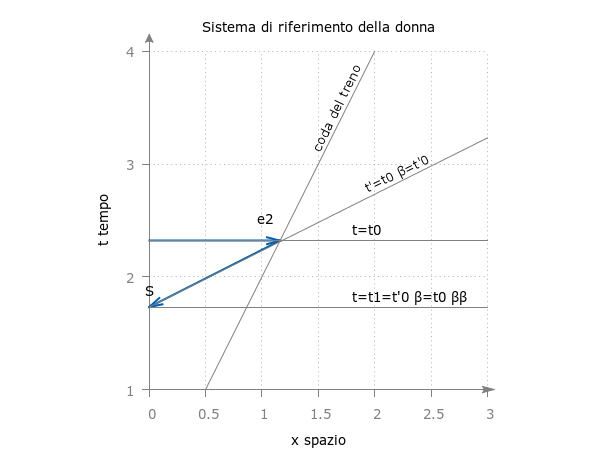
\includegraphics[scale=0.7]{figure/fig12}
 \caption{relatività galileiana}
\end{figure}

Ripercorriamo il ragionamento dal punto di vista  della signora per l'evento $e2$ tenendo d'occhio il grafico qui sopra. Vi ricordate? È il momento in cui la luce torna al passeggero.

\begin{enumerate}
 \item In $e2$ l'orologio della signora segna un certo tempo $t_0=2.32$ secondi, come sappiamo
 \item In quel momento $t_0$ il passeggero si trova in $e2$
 \item Il suo orologio in quel momento segna il tempo $t'_0 =t_0\beta=2$ che è minore di $t_0$.
\end{enumerate}

Vediamo adesso invece come stanno le cose per il passeggero:

\begin{enumerate}
 \item In $e2$ l'orologio del passeggero segna $t'_0=2$ 
 \item In $t'_0$ la signora si trova in $S$, con $x=0$ o $x'=-vt'_0$, sulla pensilina insomma
 \item In quel momento l'orologio della donna segna il tempo $t_1 =t'_1\beta$ che è minore di $t'_0$.
\end{enumerate}

Quindi bisogna sempre confrontare tra loro gli orologi che si sono sincronizzati, a parole la storiella è questa: in $e1$ la signora ed il passeggero, nello stesso punto dello spazio, sincronizzano gli orologi. Quando si verifica l'evento $e2$, ovvero la luce torna al passeggero, se la donna potesse vedere l'orologio al polso del passeggero leggerebbe un tempo minore rispetto al suo. Se quando si verifica l'evento $e2$ il passeggero potesse vedere l'orologio al polso della donna vedrebbe un orario inferiore al suo.\footnote{Da notare come questi tempi si ottengano moltiplando il precedente per $\beta$. Infatti $t_0 \beta= t'_0$ e $t'_0 \beta= t'_1 = t_0 \beta^2$. }


\section{Relatività del tempo, 4}

TODO Futuro per te, presente per me.
La simultaneità è solo dedotta, non toccata con mano.
Il figlio prima della madre? Causalità e cono di luce


\section{Misurare le lunghezze, 2}

A questo punto dovremmo essere piuttosto persuasi che il tempo possa anche essere relativo senza che il mondo sprofondi nel caos e nell'incoerenza: se ci muovessimo ordinariamente a velocità elevatissime la cosa sarebbe emersa da sempre e sarebbe forse palese per tutti.

Parlando di misura di lunghezza, qualche paragrafo più indietro, eravamo d'accordo che per una corretta misurazione gli estremi dell'oggetto devono essere considerati contemporaneamente. Nel dubbio tornate indietro a rinfrescarvi il concetto.

Però, va da sé, che se due osservatori possano non concordare sulla simultaneità, be' allora necessariamente si troveranno a non concordare sulle lunghezze.

Verifichiamo la lunghezza del treno per la donna sulla pensilina: nello stesso istante $t=0$ in cui la coda del treno la incrocia la locomotiva sarebbe $c \beta$, quindi il treno per la donna è più corto: lo spazio è relativo!

Anche in questo caso come per la velocità ed il tempo, non stiamo parlando di uno scherzo dei numeri, di un problema teorico: per entrambi gli osservatori ogni lunghezza nella direzione del movimento sarebbe più corta di quella misurata dall'altro. Se la nostra donna potesse vedere nel treno in movimento non solo vedrebbe tutto muoversi all'interno lentamente (dilatazione del tempo) ma vedrebbe anche ogni misura nella direzione del moto più corta (contrazione dello spazio), con il naso del passeggero più corto e la distanza tra la nuca ed il naso più breve. La distanza tra le spalle sarebbe invece uguale perché non si trova nella direzione del moto.

Ovviamente anche per il passeggero la donna e tutta la pensiline sarebbero più corte nella direzione del moto. Anche in questo caso non si tratta di un trucco: il treno è davvero più corto e potrebbe stare chiuso in un hangar più corto di $c$ (purché continui a muoversi, però!). 

Vediamo graficamente come passare da una misura ad un altra.

TODO Relatività delle dimensioni
%\begin{figure}[h!]
% \centering
% \includegraphics[scale=.09]{materiale/rel-distanze}
% \caption{Relatività lunghezze}
%\end{figure}


\section{Relatività Speciale}

A questo punto dovremmo avere assimilato cosa significa relatività di spazio e tempo così come intendere lo spazio-tempo: possiamo riportare tutti i dati dell'esperimento della luce con cui abbiamo introdotto il capitolo per poterlo confrontare con l'esperimento della pallina.

\begin{center}
\begin{tabular}{>{\itshape}l >{\itshape}c >{\itshape}c }
\toprule
            & \textbf{donna} & \textbf{passeggero} \\
velocità treno            & $v$        & $0$  \\ 
velocità pensilina        & $0$        & $-v$  \\
velocità pallina          & $c$        & $c$  \\
secondi dell'esperimento  & $2.32$     & $2$  \\
percorso pallina          & $2c \beta$       & $2c$  \\
lunghezza del treno       & $c\beta$   & $c$  \\
\bottomrule
\end{tabular} 
\end{center}

Sono i risultati sperimentali che portano a concepire la relatività dello spazio e del tempo. Infatti se la velocità della luce è la medesima, essendo la velocità pari allo spazio diviso il tempo, necessariamente tempi e distanze devono modificarsi proporzionalmente. Rimane invariante invece lo spazio-tempo.


\section{Conclusioni}

In queste pagine abbiamo provato a fornire una presentazione gentile ma rigorosa da un punto di vista matematico della teoria della relatività speciale di Einstein. Siamo riusciti utilizzando solo le quattro operazioni a spiegare gli effetti di dilatazione del tempo e contrazione dello spazio, ricorrendo ad un esperimento e diversi esempi. Abbiamo poi mostrato quali fossero i calcoli sottesi mostrando, in appendice, tutti i passaggi e ricorrendo a quel po' di algebra imparata in terza media.

Da qui in poi il lettore interessato potrà completare quanto appreso rinunciando alle unità di misura relativistiche e poi affrontando il non facile modello della teoria della relatività generale in cui si studiano gli effetti gravitazionali sul moto dei corpi. 


\backmatter
\appendix


\chapter{Appendice Matematica}

\section{Appendice A: la palla e il passeggero}

In questo paragrafo tutto sarà misurato dal punto di vista del passeggero sul treno. L'equazione che descrive la posizione della palla lanciata dal passeggero è:

\begin{equation} \label{eq:pass_palla} 
  x'= ct'
\end{equation}

Rispetto a lui coda e testa del treno sono ferme, in particolare la locomotiva è sempre alla stessa distanza $c$:

\begin{equation} \label{eq:pass_loco} 
  x'= c
\end{equation}

Per scoprire quando queste due traiettorie s'incontrino basta mettere a sistema le equazioni \ref{eq:pass_palla} e \ref{eq:pass_loco} sostituendo la $x'$ in entrambe:

$$ c = ct $$
$$ \frac{c}{c} = t $$
$$ 1 = t $$

Ovvero dopo un secondo. Per scoprire dove s'incontrano (ma lo sapete già vero?) basta sostituire $1$ nel tempo della \ref{eq:pass_palla} oppure nella \ref{eq:pass_loco}. 

$$ x'= ct' $$
$$ x'= c1 $$
$$ x'= c $$

Chiaramente si trovano alla distanza $c$ la distanza a cui è ferma la locomotiva. L'equazione che descrive invece il ritorno della palla è forse un po' più complessa:

\begin{equation} \label{eq:pass_palla_back} 
   x' = c(1-t') + c
\end{equation}

Ragioniamoci un istante: quando $t'=1$ il primo termine si annulla e l'equazione restituisce $c$, giustamente perché lì si trova la palla dopo un secondo. Il segno meno davanti a $t'$ ci ricorda che, questa volta, la palla si sta avvicinando al passeggero muovendosi nella direzione opposta al treno. Infine la palla continua a muoversi a velocità $c$. L'equazione del passeggero è invece facilissima visto che, dal suo punto di vista, lui non si muove affatto:

\begin{equation} \label{eq:pass_pass} 
   x' = 0
\end{equation}

Mettendo a sistema la \ref{eq:pass_pass} con la \ref{eq:pass_palla_back}:

$$ 0 = c(1-t') + c $$
$$ 0 = c -ct' + c $$
$$ ct' = 2c $$
$$ t' = 2 $$

Quindi dopo aver colpito la locomotiva passa un altro secondo e la palla è di nuovo in mano al passeggero: il cronometro segna $t'=2$, sono passati in tutto due secondi.

La pallina ha percorso una distanza pari a $c$ all'andata e $c$ al ritorno. Quindi in tutto la pallina ha percorso questa distanza:

$$\Delta x' = c+c = 2c $$

E ci ha impiegato:

$$\Delta t' = 2 $$

I calcoli ci confermano che la pallina si muove alla velocità $c$: la velocità data infatti dallo spazio percorso diviso il tempo impiegato a percorrerlo:

$$ c =\frac{\Delta x'}{\Delta t'}=\frac{2c}{c} $$


\section{Appendice B: la palla e la signora}

In questo paragrafo tutto sarà misurato dal punto di vista della donna sulla pensilina. L'equazione che descrive la posizione della palla lanciata dal passeggero è:

\begin{equation} \label{eq:donna_palla} 
  x=(c+v)t
\end{equation}


Da notare come la palla, per la donna, si muova ad una velocità superiore a $c$, per effetto della relatività galileiana. L'equazione che ci informa sulla posizione della testa del treno è:

\begin{equation} \label{eq:donna_loco} 
   x=vt+c
\end{equation}


Per sapere quando e dove il raggio raggiungerà la locomotiva basta mettere a sistema le equazioni \ref{eq:donna_palla} e \ref{eq:donna_loco}: è facile, sostituiamo la $x$:

$$ (c+v) t = vt + c $$
$$ ct+vt = vt + c $$
$$ ct = c $$
$$ t = 1 $$

Ecco la risposta, dopo un secondo la palla raggiunge la locomotiva. Dove? Basta sostituire nella \ref{eq:donna_palla} o nella \ref{eq:donna_loco} il tempo appena trovato:

$$ x=(c+v)1 $$
$$ x=c+v $$

E per tornare indietro? Come visto nel paragrafo precedente  l'equazione che descrive la traiettoria di ritorno della palla è:

\begin{equation} \label{eq:donna_palla_back} 
  x = (c-v)(1-t) + (v+c)
\end{equation}

Non è così difficile come appare, ragioniamoci un istante: quando $t=1$ ci deve restituire esattamente $v+c$ perché la palla si trova lì in quel momento. Inoltre al ritorno la palla si muove in senso contrario al treno per cui la sua velocità, per la relatività galileiana, diventa $c-v$. Infine il segno meno davanti a $t$ ci ricorda che la palla si sta avvicinando alla donna andando in direzione opposta al treno. 

L'equazione che riporta la posizione del passeggero è invece:

\begin{equation} \label{eq:donna_passeggero} 
   x = vt
\end{equation}


Come prima mettiamo a sistema le equazioni \ref{eq:donna_palla_back} e \ref{eq:donna_passeggero}:

$$ vt = (c-v)(1-t) + (v+c) $$
$$ vt = c-v -ct + vt + v+c $$
$$ vt -vt = c -ct +c +v -v $$
$$ 0 =  2c - ct  $$
$$ ct =  2c $$
$$ t =2 $$

Quindi due secondi dopo la sincronizzazione degli orologi ed un secondo dopo aver toccato la locomotiva la palla torna in mano al passeggero che, quel momento si trova in:

$$ x = vt $$
$$ x = v2 $$

Quanta distanza ha percorso la pallina? Ad andare una distanza pari a $c+v$ e  al ritorno $c-v$. Quest'ultimo dato si calcola facilmente sapendo che al secondo $1$ la pallina era nella posizione $c+v$ e nel secondo $2$ era nella posizione $2v$, per cui $c+v-2v=c-v$. Quindi in tutto la pallina ha percorso questa distanza:

$$\Delta x = c+v + (c-v) = 2c $$

E ha impiegato:

$$\Delta t = 2 $$

I calcoli ci confermano che la pallina si muove ad una velocità media di $c$ data, come sempre, dallo spazio percorso diviso il tempo impiegato a percorrerlo:

$$ c =\frac{\Delta x}{\Delta t} = \frac{2c}{2} $$


\section{Appendice C: la luce e il passeggero}

I calcoli sono li stessi presentati nella sezione La palla e il passeggero, basta sostituire la parola \textit{palla} con \textit{luce} e rammentarsi che adesso $c$ è una velocità altissima. 

\section{Appendice D: la luce e la signora}
Tutte le misure in questo paragrafo saranno riferite alla signora ferma alla banchina. L'equazione che descrive il raggio di luce emesso dal passeggero quando incrocia la donna è:

\begin{equation} \label{eq:donna_luce} 
  x=ct
\end{equation}

Da notare come tutte le stranezze derivino proprio da questa equazione: se si comportasse secondo quando indicato da galileo la luce dovrebbe andare alla velocità $c+v$ come nell'equazione \ref{eq:donna_palla}. Così non è quindi tutto prende una piega diversa.

Anche l'equazione che ci informa sulla posizione della testa del treno è invece cambiata rispetto alla  \ref{eq:donna_loco}. Vediamola
\begin{equation} \label{eq:donna_loco2} 
   x=vt+\beta c
\end{equation}

La faccenda è che misurando la lunghezza del treno\footnote{Vi ricordate come si fa vero? Si fa rimbalzare un raggio di luce e si misura quanto tempo impiega a tornare.} nell'istante in cui il passeggero incrocia la donna scopriremmo che, per questa, il treno non sia più lungo $2c$ ma $2c\beta$.  Più corto di questo fattore di contrazione $\beta$ che, data la velocità $v$, diventa una costante e , nel nostro sistema semplificato in cui $c=1$, possiamo scrivere come:

$$ \beta = \sqrt{1-v^2} $$   

Essendo $v<c=1$ anche $\beta<1$ quindi moltiplicandolo per una grandezza fisica la riduce. Nel nostro esempio il treno viaggia a $v=c/2=1/2$ per cui $\beta=0.86$. Se vi domandate da dove esca questo valore vi invitiamo ad attendere fino al prossimo paragrafo in cui sarà derivato in modo semplice, sempre con le quattro operazioni e un po' di algebra.

Tornando a noi, avendo l'equazione del raggio di luce \ref{eq:donna_luce} e quella della locomotiva \ref{eq:donna_loco2} basta metterle a sistema per sapere quando si toccheranno:

$$ ct = vt + \beta c $$
$$ ct - vt =  \beta c $$
$$ (c-v) t =  \beta c $$

\begin{equation} \label{eq:donna_deltat} 
   t = \frac{\beta c}{c-v}
\end{equation}

A questo punto possiamo sfruttare la nostra semplificazione per cui $c=1$ e la velocità del treno nel nostro esempio, $v=c/2$, per ottenere dei numeri più comodi:

$$ t = \frac{\beta}{1-\frac{1}{2}} $$
$$ t = \frac{\beta}{\frac{1}{2}} $$
$$ t = 2\beta $$

Nel nostro esempio quindi $t= 2(0.86)= 1.73 > 1$: per la donna l'intervallo di tempo che va dal momento della sincronizzazione degli orologi a quando la luce colpisce la testa del treno è maggiore di $1$ secondo. Per il passeggero invece è passato esattamente $1$ secondo!

Per trovare dove la luce colpisca la locomotiva basta sostituire la \ref{eq:donna_deltat} nella  \ref{eq:donna_luce} o nella \ref{eq:donna_loco2}:

$$ x = ct $$
$$ x = c \frac{\beta c}{c-v} $$

\begin{equation} \label{eq:donna_luce_rimb} 
  x = \frac{\beta c^2}{c-v}
\end{equation}


Ora torniamo indietro seguendo la luce nel suo viaggio di ritorno fino al passeggero. L'equazione è simile a \ref{eq:donna_palla_back} ed è questa:
 
\begin{equation} \label{eq:donna_luce_back} 
  x = c(\frac{\beta c}{c-v}-t) + \frac{\beta c^2}{c-v}
\end{equation}
 
Descriviamo le sue parti: quando $t=\frac{\beta c}{c-v}$ ci deve restituire esattamente $\frac{\beta c^2}{c-v}$ perché la luce si trova, in quel momento, in quel punto (come stabilito dalla \ref{eq:donna_luce_rimb}). Inoltre al ritorno la luce si muove in senso contrario al treno ma la sua velocità è sempre, ostinatamente, $c$! Infine il segno meno davanti a $t$ ci ricorda che la luce si sta avvicinando alla donna. 

L'equazione del passeggero è invece sempre:

$$ x=vt $$

Quindi mettendo a sistema questa con la \ref{eq:donna_luce_back} otteniamo:

$$ vt = c(\frac{\beta c}{c-v}-t) + \frac{\beta c^2}{c-v}  $$
$$ vt = \frac{\beta c^2}{c-v} – ct + \frac{\beta c^2}{c-v} $$
$$ vt + ct = \frac{2\beta c^2}{c-v} $$
$$ (v + c)t = \frac{2\beta c^2}{c-v} $$   
$$ t = \frac{2\beta c^2}{(c-v)(v+c)} $$   
$$ t = \frac{2\beta c^2}{c^2-v^2} $$

Bene, ci siamo quasi: nel nostro mondo semplificato $c=1$ e ricordo che $1-v^2=\beta^2$, per cui:

$$ t = \frac{2\beta}{1-v^2} $$
$$ t = \frac{2\beta}{\beta^2} $$
$$ t = \frac{2}{\beta} $$

Nel nostro esempio quindi $t= 2/0.86= 2.32 > 2s$: quindi anche nell'esperimento completo il raggio di luce impiega $2$ secondi per il passeggero e $2.32$ secondi per la donna.

Concludiamo con i soliti conti circa spazio, tempo e velocità. La luce ha percorso una distanza pari a $\frac{2c}{\beta}$. In effetti è facile da verificare visto che la luce si muove sempre a velocità $c$ e sono passati in tutto $\frac{2}{\beta}$ secondi. 

Si può notare già vedere in azione il fattore di conversione di intervalli di tempo e di spazio: se vi ricordate il treno è lungo $2c$ per il passeggero ma solo $2c\beta$ per la donna. Analogamente la distanza percorsa in tutto dalla luce, come si è appena visto, è $\frac{2c}{\beta}$ per la donna e $2c$ per il passeggero, così come il tempo è $\frac{2}{\beta}$ per la donna e $2$ per il passeggero. Si tratta di moltiplicare per $\beta$, come farlo in modo corretto è spiegato nel paragrafo TODO.

  


%%% BIBLIOGRAPHY
%%% -------------------------------------------------------------

% \bibliographystyle{utphysics}
% \bibliography{ref}

\end{document}
